\documentclass[11pt]{article}

% ===========================================================================
% timbreprobe — Stage 0 paper draft (expanded)
% Compile:  pdflatex main && pdflatex main       (two passes)
% Numbers that depend on the seed-0 E2 run come from the macros below;
% regenerate them with the commands listed in Appendix E.
% ===========================================================================

\usepackage[a4paper,margin=2.6cm]{geometry}
\usepackage{graphicx}
\usepackage{booktabs}
\usepackage{amsmath,amssymb}
\usepackage[T1]{fontenc}
\usepackage[utf8]{inputenc}
\usepackage{lmodern}   % scalable fonts (needed by microtype font expansion)
\usepackage{microtype}
\usepackage{hyperref}
\usepackage{xcolor}
\usepackage{caption}
\usepackage{enumitem}
\usepackage{array}

\hypersetup{colorlinks=true,linkcolor=blue!50!black,citecolor=blue!50!black,
            urlcolor=blue!60!black}
\captionsetup{font=small,labelfont=bf}
\setlist{nosep,leftmargin=1.4em}
\setlength{\emergencystretch}{3em}   % long \code{} names cannot hyphenate
\sloppy

% code names: \code{grad_surrogate} works without escaping underscores
\newcommand{\code}[1]{\texttt{\detokenize{#1}}}

% a numbered pseudocode block (no extra packages needed; body may be verbatim)
\newcounter{algcounter}
\newenvironment{alg}[1]{\par\medskip\refstepcounter{algcounter}%
  \noindent\textbf{Algorithm \thealgcounter: #1}\par\nopagebreak\small\medskip}%
  {\medskip}

% ---------------------------------------------------------------------------
% RESULTS NUMBERS — single source of truth (seed-0 smoke run)
% ---------------------------------------------------------------------------
\newcommand{\nTarg}{48}
\newcommand{\nHold}{24}
\newcommand{\nDrop}{43}
\newcommand{\nInit}{2.74}
\newcommand{\nRand}{4.08}
\newcommand{\rRetU}{1.45}
\newcommand{\rGS}{2.59}
\newcommand{\rGST}{1.36}
\newcommand{\rGR}{1.60}
\newcommand{\rGT}{0.875}
\newcommand{\rGTci}{[0.81, 0.92]}
\newcommand{\rCMA}{1.00}
\newcommand{\rCMAci}{[0.90, 1.00]}
\newcommand{\nGTfin}{2.35}   % median final distance, oracle
\newcommand{\nCMAfin}{2.65}  % median final distance, CMA-ES
\newcommand{\renGT}{5\,856}
\newcommand{\renCMA}{21\,696}
\newcommand{\renGR}{528}
\newcommand{\succGT}{0.06}
\newcommand{\succCMA}{0.06}
% seed-1 replication
\newcommand{\sOneGT}{0.877}
\newcommand{\sOneCMA}{1.000}
\newcommand{\sOneGS}{2.313}
\newcommand{\sOneGST}{1.376}
\newcommand{\sOneGR}{1.475}
\newcommand{\sOneRetU}{1.499}

\title{\bfseries Probing Timbre Space:\\ Gate Experiments for Inverse Synthesizer Patch Synthesis}

\author{Feng Yuhan\thanks{%
  Independent Researcher.  \texttt{fengru1005@gmail.com}.
  Code, data and the listening-test generator:\\
  \url{https://github.com/Fengrru/timbreprobe}}}

\date{Draft --- \today}

\begin{document}
\maketitle

% ===========================================================================
\begin{abstract}
\noindent
A system that turns human intent---a text description or a hummed
melody---into a \emph{structured synthesizer parameter set} (a patch) rather
than audio must clear two assumptions before it is worth building: (i) an
embedding distance between two sounds has to track human similarity
judgements, and (ii) that distance has to be usable as an objective function
for search over patch parameters. We treat these as \emph{gate hypotheses},
build a testbed that can falsify them at low cost, and report what it says.

The testbed (\emph{timbreprobe}) consists of a differentiable subtractive
synthesizer (31 parameters, STFT-domain time-varying filtering,
bit-deterministic renders), an 85-dimensional differentiable DSP embedding, an
anchor-stratified corpus of 3{,}895 patches of which four entire anchor regions
are held out, a learned patch\,$\rightarrow$\,embedding surrogate, and seven
search strategies that all start from the same retrieval-based initialisation
per target.

On the navigability gate the answer is \emph{weakly positive}, and the way it
fails is the informative part. True-gradient search is the only method that
beats its retrieval start (median distance ratio \rGT, 95\% CI \rGTci), but it
plateaus after roughly 15\% and consumes \renGT{} real renders. A
derivative-free baseline (separable CMA-ES) spends $3.7\times$ more renders and
makes no measurable progress at all (\rCMA: its median target is unchanged).
All three surrogate-based strategies end \emph{worse than not searching}
(ratio \rGST--\rGS), and---the diagnostic signature---they
degrade \emph{more} in-distribution than on held-out targets, i.e.\ the
optimiser exploits surrogate error precisely where the surrogate is most
confident. Surrogate distance-rank fidelity falls from Kendall $\tau=0.70$
in-distribution to $0.39$ on unseen regions, while the true-gradient oracle is
unaffected. The bottleneck is therefore the surrogate, not the search
algorithm; the dominant failure mode is extrapolation plus exploitation rather
than interpolation error.

We release the testbed, the pre-registered listening-test material for the
empirical gate, and a roadmap in which every subsequent stage has an explicit
gate and a falsification criterion. Six engineering findings that cost real
time are documented---a per-sample IIR loop is $100\times$ slower than an
equivalent spectral formulation, multi-threaded torch can be $2$--$5\times$
slower than single-threaded at these tensor shapes, \code{torch.istft} backward
produced non-finite gradients at padded edges, an \code{asin}-based triangle LFO
has an infinite derivative at its extrema, fixed-step Adam overshoots by
$1.7\times$ in distance within five steps, and a corpus jitter layer can place
test patches within numerical noise of training patches, which makes the
improvement ratio degenerate unless targets are filtered.
\end{abstract}

% ===========================================================================
\section{Introduction}\label{sec:intro}

\paragraph{The problem.}
Building a sound is a search problem. A producer who wants ``a warm detuned pad
with a slow filter opening'' does not know which of a modern synthesizer's
several hundred parameters to move; they iterate, listening between attempts.
Recent products automate parts of that loop. Fadr's \emph{SynthGPT~2} accepts a
text description and returns a playable patch, with a human listening between
candidates; Sonic~Charge's \emph{Genopatch} evolves patches toward an imported
audio sample \cite{fadr,genopatch}. Both are impressive, and both are
\emph{closed-loop without a perceptual objective}: the machine proposes, a human
decides, and nothing in the system knows \emph{why} one candidate was preferred.

Our larger goal is a system that maps human intent---text, a humming reference,
or both---to a patch, and that can improve from listening feedback rather than
only from a human gate. Architecturally that requires two things before any
generative machinery is justified.

\begin{description}[leftmargin=1.2em]
\item[Assumption A (perceptual monotonicity).] There exists an embedding space
  of audio in which distance predicts human similarity judgements for timbre,
  at least ordinally. If not, ``optimising toward a target embedding'' is
  optimising toward nothing.
\item[Assumption B (navigability).] Given a target in that space, a search
  procedure can find patch parameters that reach it, at a render budget a user
  would tolerate. If not, the loop must be retrieval-and-rerank only.
\end{description}

This paper tests A and B \emph{before} building the system, and reports what the
tests revealed. We deliberately chose a testbed whose oracle is exact---a
differentiable synthesizer---so that ``true gradient'' navigation is available
as an upper bound and render budgets can be accounted for honestly. This turned
what we expected to be a calibration exercise into a result: the naive design
(learn a surrogate, optimise freely on it) fails, and it fails in a way that is
measurable, diagnosable, and cheap to detect in advance.

\paragraph{Contributions.}
\begin{enumerate}[label=(\arabic*)]
\item A \emph{differentiable timbre testbed}: a 31-parameter subtractive
  synthesizer whose time-varying filter is implemented in the STFT domain
  (validated against a per-sample state-variable reference at Spearman
  $\rho=0.996$), with bit-deterministic renders and an 85-dimensional
  differentiable DSP embedding, giving an exact oracle for
  patch\,$\rightarrow$\,percept gradient navigation at CPU-feasible cost
  (\S\ref{sec:testbed}).
\item A \emph{gate protocol} with three experiments: E2 (navigability, fully
  automatic), E3 (surrogate fidelity, reported per \emph{region} rather than in
  aggregate), and E1 (a pre-registered triplet 2AFC listening test whose
  material the code generates; human data pending) (\S\ref{sec:protocol}).
\item \emph{Negative results with a signature}: all surrogate-based search
  degrades below the no-search baseline, and the degradation is largest where
  the surrogate is most confident---a measurement that costs one extra data
  split, and that we recommend as a standard diagnostic
  (\S\ref{sec:res-surrogate}).
\item A \emph{render-efficiency comparison} showing that gradient information
  beats population search by more than $3\times$ in render budget at this
  dimensionality, which argues for investing in differentiable proxies rather
  than larger populations (\S\ref{sec:res-pareto}).
\item \emph{Diagnostics that localise the failure}: a residual
  decomposition, a discrete-jump correlation, an ablation of the monotone
  accept rule, and a block-balanced-metric control
  (\S\ref{sec:res-diagnostics}). Together they rule out the accept rule as
  the binding constraint, show that the leftover error is spread across the
  objective roughly in proportion to dimensionality (per-dimension shares
  $0.85$--$2.34\times$ uniform, i.e.\ only mildly overweighted in the
  discrete-sensitive blocks), and motivate re-weighting or learning the metric
  rather than a more elaborate search.
\item \emph{A documented corpus trap}: a jitter-sampled corpus places
  $\sim$4\% of test patches within numerical noise of training patches, making
  the improvement ratio unbounded for those targets; the fix (a scale-free
  minimum target distance) and its effect on reported means are described in
  \S\ref{sec:targets}.
\item An \emph{evidence-linked roadmap} (\S\ref{sec:roadmap}) in which every
  next step is tied to the observation that motivates it and to a criterion
  that would falsify it.
\end{enumerate}

% ===========================================================================
\section{Related work}\label{sec:related}

\subsection{Inverse synthesis and preset generation}

Learning to map from sound to synthesizer control has a long history, from
flow-based synthesis of parameters from audio \cite{flow} to differentiable
digital signal processing, where a differentiable synthesizer is placed inside
the training loop \cite{ddsp}. Percussive audio has been mapped to synthesizer
parameters in real time with a differentiable drum synthesizer
\cite{timbreremap}, and the non-proportional geometry between synth parameters
and their perceptual effect has been studied directly \cite{synthmaps}.
Commercially, \emph{Genopatch} evolves patches toward a target sample by genetic
search in parameter space \cite{genopatch}, and \emph{SynthGPT~2} generates
patches from text with a human in the loop \cite{fadr}.

Two things distinguish our work from this line. First, it does not propose a
generator: it asks what an honest objective for such a generator must look like,
and measures the cost of getting it wrong. Second, its evaluation protocol
forces all methods to start from the same retrieval point, which changes the
conclusions one draws about how much optimisation is worth (see
\S\ref{sec:res-pareto} and \S\ref{sec:disc-retrieval}).

\subsection{Perceptual embeddings for timbre, and their validation}

Wessel's timbre space established that timbre is navigable in a low-dimensional
perceptual geometry \cite{wessel}, but the coordinates were hand-designed.
Modern audio--text and music representation models---CLAP \cite{clap}, MERT
\cite{mert}, MuQ \cite{muq}---provide learned spaces in which distance is often
\emph{assumed} to be perceptually meaningful. Our E1 protocol is a way to test
that assumption for timbre specifically, and our testbed deliberately keeps a
handcrafted embedding as a lower anchor: a pretrained model that cannot beat
handcrafted spectral features on human similarity judgements is not a
perceptual model for this task, whatever its retrieval benchmarks say.

\subsection{Surrogates, trust regions, and model exploitation}

Optimising a learned model of an expensive objective is standard practice, and
so is its central failure mode: the optimiser finds regions where the model is
wrong \cite{turbo}. Trust-region methods constrain the search to where the model
is locally valid \cite{turbo}; our E2 result quantifies the same phenomenon in a
perceptual setting, shows that the damage is \emph{larger} in-distribution than
out-of-distribution (the signature of exploitation rather than mere
generalisation error), and shows that a trust region recovers only part of the
loss. For derivative-free comparison we use separable CMA-ES \cite{sepcma}
within the CMA-ES family \cite{cmakes}; gradient search uses Adam \cite{adam}.

\subsection{Humming and intent}

Humming as a query is attractive because it carries pitch and articulation
directly. But its \emph{source} is a human voice while the target is a
synthesizer, so a na\"ive audio embedding answers ``imitate this singer''---the
wrong question. The roadmap therefore treats humming as an
intent-factorisation problem rather than audio-to-audio matching: pitch
trajectory $\rightarrow$ tuning parameters; posture (attack sharpness, vibrato
rate and depth, legato) $\rightarrow$ envelopes and LFO; brightness and vowel
colour $\rightarrow$ filter and drive (\S\ref{sec:roadmap}).

% ===========================================================================
\section{The \emph{timbreprobe} testbed}\label{sec:testbed}

\subsection{Design constraints}

A gate experiment needs its oracle to be exact, its cost to be accounted, and
its conclusions to be attributable. We therefore build the synthesizer rather
than adopting one:

\begin{itemize}
\item \textbf{Exact gradients.} Because the entire chain
  parameter\,$\rightarrow$\,audio\,$\rightarrow$\,embedding is differentiable,
  ``true gradient'' navigation is available as an upper bound that no surrogate
  can exceed. Without it, a failed surrogate experiment cannot be distinguished
  from a hard landscape.
\item \textbf{Render accounting.} Every real render is counted, so methods can be
  compared by \emph{quality per render} rather than per iteration---the resource
  a practical system actually spends.
\item \textbf{Controlled difficulty.} A 31-parameter space is small enough that
  a corpus can cover it in layers and large enough to contain the phenomena of
  interest (coupled parameters, discrete choices, log-scaled axes).
\item \textbf{Determinism.} Renders are bit-identical for identical patches
  (fixed noise seed), which the search methods rely on.
\end{itemize}

The cost of this choice is realism: our synthesizer is not a specific
commercial instrument, has no effects section, and filters without phase
response (\S\ref{sec:filter}). It is an oracle for gate hypotheses, not a
substitute for a target instrument; \S\ref{sec:roadmap} makes the port to a real
instrument an explicit, gated phase.

\subsection{Parameter schema and its representation}\label{sec:schema}

The synthesizer exposes $D=31$ parameters (Table~\ref{tab:schema} in
Appendix~\ref{app:schema}). The optimiser always works in the unit hypercube
$u \in [0,1]^{D}$; physical units are recovered by

\begin{equation}
\text{linear:}\quad v = \ell + u\,(h - \ell), \qquad
\text{log:}\quad v = \ell\,(h/\ell)^{u},
\end{equation}

where $\ell,h$ are the physical bounds. Log scaling is used for the cutoff, $Q$,
and the envelope times and LFO rate, because a factor of two in cutoff is a
perceptually equal step everywhere while an additive step is not.

Discrete parameters (waveform, octave, filter type, LFO target and waveform, and
the pulse-duty choice) are represented as a continuous \emph{position} over the
ordered choice list. With $k$ choices and $p = u\,(k-1)$,

\begin{equation}
w_j = \frac{\max\left(0,\,1 - |p - j|\right)}{\sum_{j'}\max(0, 1 - |p - j'|)},
\qquad
\hat\theta = \sum_j w_j\,\theta_j,
\label{eq:choice}
\end{equation}

i.e.\ a piecewise-linear morph between adjacent choices, and the \emph{hardened}
patch used for reporting is $j^\star = \mathrm{round}(p)$.

This choice of kernel, rather than a softmax or Gumbel relaxation, is
deliberate. Real preset patches sit exactly \emph{on} a choice, and a softmax
kernel's derivative vanishes there, which would freeze discrete dimensions for
gradient search at the very points where the corpus is dense. The triangular
basis satisfies $|\partial w_j/\partial p| = 1$ throughout and is a partition of
unity on $[0, k-1]$, so gradients stay alive everywhere and the parameter reads
as an interpretable morph knob.

\subsection{Signal chain}\label{sec:chain}

The chain is
\begin{equation}
\text{osc}_1(\text{+PM}) + \text{osc}_2 + \text{sub} + \text{noise}
\;\rightarrow\; \text{drive} \;\rightarrow\; \text{filter} \;\rightarrow\;
\text{VCA} \;\rightarrow\; \text{master} \;\rightarrow\; \text{RMS},
\end{equation}
rendered at $f_s = 16$\,kHz for 0.25\,s on a fixed C4 ($261.63$\,Hz).

\paragraph{Oscillators.} Each oscillator is additive over $K=24$ harmonics with
per-family unit-RMS coefficient vectors:
\begin{equation}
a^{\text{sine}}_1 = 1;\quad a^{\text{saw}}_k = \tfrac{1}{k};\quad
a^{\text{tri}}_k = \tfrac{1}{k^2}\ (k\ \text{odd});\quad
a^{\text{pulse}}_k(d) = \tfrac{2}{k\pi}\sin(\pi k d),
\end{equation}
normalised so that $\sum_k a_k^2/2 = 1$. The families are blended with the
weights of Eq.~\eqref{eq:choice}, and each harmonic is masked to prevent
aliasing at the render pitch:
\begin{equation}
m_k = \sigma\!\left(\frac{0.95 f_{\text{Nyq}} - k f_0 (1 + 0.6\,\text{FM})}
{0.05 f_{\text{Nyq}}}\right),
\qquad
o(t) = \sum_{k=1}^{K} m_k a_k \sin\!\big(k\,\phi(t)\big),
\label{eq:osc}
\end{equation}
with phase obtained by integrating the instantaneous frequency and adding phase
modulation,
\begin{equation}
\phi(t) = \frac{2\pi}{f_s}\sum_{\tau \le t} f(\tau) + I\, o_2(t),\qquad
f(t) = f_{C4}\, 2^{\,\text{oct} + \text{cents}/1200}\, \cdot\,
2^{\,w_{\text{pitch}} D_{\text{LFO}}\, 7\, \text{LFO}(t)/12}.
\end{equation}
All harmonic phases are sine phases: the embedding is magnitude-based and thus
phase-invariant, and the ear is largely phase-insensitive for steady tones, so
this costs nothing here and keeps the synthesis differentiable. The sub
oscillator is a sine one octave below oscillator 1 (i.e.\ at $f/2$); noise is a
white/pink blend, the pink component shaped as $1/\sqrt{f}$ in the frequency
domain from a fixed-seed white signal.

\paragraph{Modulation and envelopes.} The LFO is a closed-form waveform set---
sine, triangle $1 - 4\,|\mathrm{frac}(\varphi{+}0.25) - 0.5|$, softened square
$\tanh(6\sin 2\pi\varphi)$, saw $2\,\mathrm{frac}(\varphi)-1$---blended with
Eq.~\eqref{eq:choice} and routed to cutoff ($\pm3$ octaves), pitch
($\pm7$ semitones) or amplitude (tremolo depth 0.5). Envelopes (filter and
amplitude) are
\begin{equation}
\mathrm{env}(t) = \begin{cases} t/a, & t < a,\\[2pt]
s + (1-s)\,e^{-(t-a)/\tau_d}, & t \ge a,\end{cases}
\qquad \tau_d = d/5,
\label{eq:env}
\end{equation}
a linear attack into an exponential decay, continuous at $t=a$ and
differentiable everywhere except that single point.

\paragraph{Filter, VCA, output.} The filter is a time-varying state-variable
filter, described in \S\ref{sec:filter}. The VCA multiplies by
$\mathrm{env}_a(t)$ and the tremolo, the output stage applies
$\tanh(g_m \cdot y)$ with $g_m \in [1,8]$, and the render is finally
RMS-normalised to $0.1$, so loudness is not a distance cue (mirroring loudness
matching in listening tests).

\subsection{Filtering in the STFT domain}\label{sec:filter}

A per-sample zero-delay-feedback state-variable filter \cite{zavalishin} was the
first implementation, and it was unusable: \textbf{10\,s per batch forward and
60\,s with backward}, essentially independent of batch size, because 6400
Python-level iterations dominate. We therefore apply the \emph{analytic
magnitude response} of the same filter family once per STFT frame
($n_{\text{fft}}=256$, hop $64$, i.e.\ 4\,ms control rate):
\begin{equation}
r = \frac{f}{f_c(\text{frame})},\qquad
|H_{lp}| = \big[(1-r^2)^2 + (r/Q)^2\big]^{-1/2},\qquad
|H_{hp}| = r^2|H_{lp}|,\qquad |H_{bp}| = \frac{r}{Q}|H_{lp}|,
\label{eq:svf}
\end{equation}
with LP/HP/BP and 12\,/\,24\,dB/oct as soft blends
($H = (1-\lambda)H_{12} + \lambda H_{12}^2$), and the per-frame cutoff
\begin{equation}
f_c(t) = \mathrm{clamp}\Big(f_{c0}\; 2^{\,A_e\,\mathrm{env}_f(t)\,5}\;
2^{\,w_{\text{cut}} D_{\text{LFO}}\,3\,\mathrm{LFO}(t)},\; 20,\; 0.92 f_{\text{Nyq}}\Big).
\end{equation}
Synthesis uses a hand-rolled overlap-add with a clamped window-envelope
normaliser (not \code{torch.istft}, whose backward divides by a near-zero
envelope at the padded edges and produced non-finite gradients).

\paragraph{What this costs, and why the experiments survive it.}
The substitution preserves per-frame time-varying cutoff, the $Q$ peak, and the
type/slope blends. It removes the filter's \emph{phase} response: no ringing, no
self-oscillation, and spectral transients are smoothed at the 16\,ms analysis
window. Three design decisions limit the consequences. (i) The amplitude
envelope is applied \emph{after} synthesis, so loudness transients---what the
envelope features measure---stay sample-accurate. (ii) Every embedding
dimension is a magnitude or an envelope statistic; none depends on phase.
(iii) The engineering claim is validated directly: on a fixed test signal the
spectral filter's log-magnitude spectrum agrees with the per-sample reference at
Spearman $\rho = 0.996$ (checked by \code{sanity}). What a real instrument port
must re-check is exactly the part we removed---transient bite and resonance
character---which is why \S\ref{sec:roadmap} makes the port a separate gated
phase rather than an assumption.

\subsection{The embedding}\label{sec:embedding}

The embedding is 85 handcrafted, differentiable dimensions, grouped into 13
blocks (Appendix~\ref{app:features}): 32 log-mel bands with mean and standard
deviation (64 dims), spectral centroid, bandwidth, soft rolloff, flatness, flux
and slope (mean/std each), crest factor, a high/low band ratio, four envelope
statistics, a smooth zero-crossing proxy, and harmonic and odd/even harmonic
ratios referenced to the patch's fundamental. Features are $z$-scored with
corpus statistics.

Two properties are engineered deliberately.

\paragraph{Smoothness.} Every hard, non-differentiable operation is replaced by
a smooth surrogate, because a feature with zero gradient almost everywhere
contributes nothing to gradient navigation while still distorting distances:
the rolloff threshold becomes a sigmoid weighting
($w_f = \sigma((\mathrm{cum}_f - 0.85\,\mathrm{tot})/(0.05\,\mathrm{tot}))$),
the envelope's peak position becomes a log-sum-exp, and the zero-crossing rate
becomes $\tfrac{f_s}{2}\langle \sigma(-x_t x_{t+1}/\sigma_x^2)\rangle$ with
$\sigma_x^2 = 0.05\langle x^2\rangle$.

\paragraph{Harmonic structure.} Two dimensions are computed against the patch's
own fundamental $f_0$ via Gaussian combs
$w^{(k)}_f = \exp(-((f - k f_0)/(0.35 f_0))^2)$: the total energy captured by
the comb (harmonicity) and the odd-to-even ratio (which separates square- from
saw-family timbres). These are the dimensions most sensitive to \emph{discrete}
choices, and they matter in the diagnostics of \S\ref{sec:res-diagnostics}.

The embedding plays two roles: it is the objective for E2, and it is the
\emph{lower anchor} for E1---a pretrained embedding that cannot beat it on human
judgements is not worth adopting. It is not claimed to be perceptual.

\subsection{Corpus construction}\label{sec:corpus}

Uniform random sampling of a 31-dimensional synth space is a poor corpus: most
of the volume is perceptually degenerate (nothing audible; everything wide
open). The corpus is built in layers around 16 hand-designed anchors with
semantic labels (bright lead, warm pad, dark sub, hollow square, narrow pulse,
FM brass, noise breath, pluck, resonant sweep, soft flute, triangle organ, HP
air, octave stack, sub-heavy pad, driven lead, metallic FM), of which \emph{four
are held out entirely} and serve as generalisation probes:

\begin{itemize}
\item \emph{sweeps}: for every anchor and every dimension, three values moved
  across the range with the anchor fixed ($31 \times 3 \times 16$,
  deduplicated)---these map each axis's \emph{local} perceptual direction;
\item \emph{jitter}: 120 Gaussian perturbations per anchor
  ($\sigma = 0.10$ continuous, $0.03$ choice, so patches stay close to ``hard''
  presets)---these populate the neighbourhoods optimisation actually traverses;
\item \emph{uniform} (500) and \emph{sparse} (150, one or two sources active)
  for global coverage.
\end{itemize}

After deduplication on rounded coordinates this yields 3{,}895 unique patches,
split into train 2{,}468 / val 308 / test 1{,}119 (of which 811 belong to the
held-out anchor regions). The corpus is a scientific instrument: neutral and
controlled. A Stage-1 retrieval library would instead use \emph{real} factory
presets, where a biased distribution is a feature, not a bug.

\paragraph{A corpus trap worth reporting.} Because the jitter layer is dense,
some test patches land within numerical noise of a training patch: in the smoke
corpus, \nDrop{} of roughly one thousand test candidates have a
nearest-training-neighbour distance below a quarter of the median, and a few are
numerically \emph{identical} to a training patch. Such targets are already
solved by the retrieval start, so their ``improvement'' ratio
$d_{\text{final}}/d_{\text{init}}$ is unbounded---left in, three such targets
dragged the \emph{mean} ratio of every method to $\sim 10^{7}$ while leaving
medians untouched. E2 therefore rejects targets closer than
$0.25\times$ the median nearest-neighbour distance and resamples
(\S\ref{sec:targets}). Anyone building a sampled patch corpus should check for
this before reporting ratio means.

\subsection{Render protocol and identifiability}\label{sec:identifiability}

The protocol is a single 0.25\,s sustained C4, no note-off. This makes the
comparison clean (every patch is heard as the same note, so ``timbre'' is
isolated from ``melody'') and it makes the experiment cheap, at the price of
identifiability. Table~\ref{tab:ident} states what is and is not recoverable;
parameter-recovery numbers must be read against it.

\begin{table}[t]
\centering\small
\caption{Identifiability under the render protocol.}
\label{tab:ident}
\begin{tabular}{p{5.1cm}p{9.6cm}}
\toprule
not identifiable & why \\
\midrule
envelope release stages & no note-off in the protocol \\
slow LFOs (below $\sim$4\,Hz) & less than one cycle in 0.25\,s \\
absolute loudness & render is RMS-normalised \\
source level, if it is the only & level is absorbed by the normaliser \\
\quad active source & \\
oscillator\,2 amplitude under FM & FM index and level trade off \\
\bottomrule
\end{tabular}
\end{table}

% ===========================================================================
\section{Experimental protocol}\label{sec:protocol}

\subsection{E2: navigability}\label{sec:e2}

\paragraph{Targets and the shared start.}\label{sec:targets}
All methods start each target from the \emph{same} point: the nearest
\emph{training} patch in embedding space---the retrieval initialisation a
practical system would use. \nTarg{} targets are sampled from the test split,
deliberately balanced (\nHold{} from held-out anchor regions, the rest
in-distribution) so that generalisation is measured rather than assumed, and
filtered against near-duplicates as described in \S\ref{sec:corpus}. Every
reported number is therefore the value added \emph{on top of retrieval}; a
method that cannot beat its own start point has negative value.

\paragraph{Methods.}
\begin{itemize}
\item \code{retrieval_nearest} --- the start point itself (ratio 1.000 by
  construction);
\item \code{retrieval_unigram64} --- best of 64 random training presets, the
  ``blind trial-and-error'' floor;
\item \code{grad_surrogate} --- adaptive-step gradient search on the learned
  surrogate (200 steps, zero renders during search);
\item \code{grad_surrogate_trust} --- the same, confined to an $L_2$ ball of
  radius $0.35$ around the start;
\item \code{grad_reground} --- surrogate search with re-grounding: every 20
  steps the current patches are rendered for real and the surrogate copy is
  fine-tuned online (10 rounds);
\item \code{cmaes_true} --- separable CMA-ES \cite{sepcma} on the true
  objective (45 generations, population 10);
\item \code{grad_true} --- the oracle: adaptive-step gradient search through the
  real renderer (60 steps).
\end{itemize}

\paragraph{Optimiser detail that matters.}
Fixed-step Adam diverges on this objective: at $\eta = 0.05$ the \emph{true}
distance rose from $3.08$ to $5.29$ within five steps and never recovered. The
space is 31-dimensional with log-scaled axes (a $0.1$ change in the cutoff
coordinate is a $2.4\times$ change in Hz), so any fixed step is either far too
large or uselessly small. All gradient methods therefore keep the Adam direction
and adapt the step \emph{per target}: a candidate is accepted only if it does
not increase the objective, with the step growing $1.3\times$ on success and
halving on failure, bounded to $[\eta/64, 4\eta]$. This costs one extra
objective evaluation per step and no gradient. The full loop is
Algorithm~\ref{alg:step}.

\begin{alg}{Adaptive-step gradient navigation (per target, batched)}\label{alg:step}
\begin{verbatim}
in:  start patches u0, target embeddings z*, steps n, initial step eta
     d <- J(u0);   lr <- eta
     for t = 1..n:
         g   <- grad_u || S(u) - z* ||           # S = renderer or surrogate
         dir <- Adam(g)                          # bias-corrected direction
         c   <- clip(u - lr * dir, 0, 1)
         if trust_radius > 0: c <- project_ball(c, u0, trust_radius)
         d_c <- J(c)                             # one objective evaluation
         take   <- (d_c <= d) if monotone else True
         u      <- take ? c : u;   d <- take ? d_c : d
         lr     <- lr * (d_c <= d ? 1.3 : 0.5)   # bounded to [eta/64, 4*eta]
     return u
--------------------------------------------------------------------
J(x) = || S(x) - z* || : L2 distance in the z-scored embedding space.
S is the real renderer (renders counted) or the learned surrogate (free).
\end{verbatim}
\end{alg}

\paragraph{Re-grounding.}\label{sec:reground}
\code{grad_reground} starts from the trained surrogate, runs 20 surrogate steps,
then renders the current patches for real, appends them to a replay buffer
(initialised with 256 training patches) and fine-tunes its surrogate copy for 15
inner Adam steps at $\mathrm{lr}=3\times10^{-4}$; this repeats for 10 rounds. It
is the minimal implementation of the ``learned surrogate accelerates, DSP
validates'' loop, and its render cost (\renGR{} patch renders) is reported
against the others.

\paragraph{Metrics.}
$\text{ratio} = d_{\text{final}}/d_{\text{init}}$ per target, reported as its
median with a bootstrap 95\% CI (2{,}000 resamples over targets). We also report
success rates at ratio $<0.5$ and $<0.2$, the median absolute reduction
$d_{\text{init}} - d_{\text{final}}$ (well defined even if a start distance is
near zero), hardened parameter recovery L1, real renders consumed, and wall
time---all split by regime (in-distribution vs held-out anchors).

\subsection{E3: surrogate fidelity}\label{sec:e3}

The surrogate is an MLP ($31 \rightarrow 256 \rightarrow 256 \rightarrow 85$,
GELU, Adam at $10^{-3}$, batch 256, early stopping on the validation split with
patience 40). We report $R^2$ and cosine per split \emph{and} the distance-rank
correlation (Kendall $\tau$ over pairwise embedding distances, computed with the
Gram-identity pairwise form to avoid an $[N,N,D]$ temporary), because rank
agreement is what a search procedure actually consumes.

\subsection{E1: perceptual monotonicity (pre-registered; human data pending)}\label{sec:e1}

\code{python -m timbreprobe.cli e1} samples a 600-patch pool, re-renders it at
0.5\,s and re-embeds \emph{that} audio, so listeners judge exactly the audio the
distances were computed on. Each trial plays a reference A and two options whose
embedding distances to A fall in \emph{different quantile bins} of the pool's
distance distribution (measured bin edges for the smoke pool: 7.18 / 10.26 /
14.05); the closer option's screen position is randomised; the page never
contains the answer key; 120 triplets per listener. Analysis reports agreement
per contrast level with Wilson intervals.

\emph{Pre-registered gate.} The primary embedding must agree with listeners
above chance with a 95\% Wilson interval excluding $0.5$, \emph{and} agreement
must increase monotonically with contrast strength. A pretrained embedding
replacing the handcrafted one must additionally beat it on the same trials.

\subsection{Diagnostics and replication}\label{sec:diagprotocol}

Three additions beyond the gate protocol itself, all cheap and all reported in
\S\ref{sec:res-diagnostics}:

\begin{itemize}
\item \textbf{Residual decomposition.} After oracle navigation, split the
  remaining squared distance into the embedding's 13 blocks:
  $\mathrm{share}_B = \mathbb{E}_m\big[\sum_{j\in B}\delta_{mj}^2 /
  \sum_j \delta_{mj}^2\big]$ with $\delta = z_{\text{final}} - z^\star$.  Concentration in the
harmonic blocks---the ones that respond to discrete
  choices---would be direct evidence for the discrete-jump reading of the
  plateau; as \S\ref{sec:res-diagnostics} reports, the measured concentration
  is mild ($2.3\times$ uniform per dimension for the harmonic block, while the
  64-dimensional log-mel block absorbs $72\%$ of the residual simply because of
  its size).
\item \textbf{Discrete-jump correlation.} For each target, count how many
  discrete dimensions differ (hardened) between the start patch and the target
  patch, and correlate that count with the achieved ratio (Spearman).
\item \textbf{Monotone ablation.} Re-run the identical search with
  \code{monotone=False} (every candidate accepted; adaptive step kept) at the
  same budget. Only a non-monotone walk can cross a valley, which is what a
  discrete jump requires; if the free walk does not improve things, the
  landscape---not the rule---is the constraint.
\item \textbf{Seed replication.} The full E2 protocol is re-run with seed 1
  (different surrogate initialisation, different target sample, same corpus).
\end{itemize}

% ===========================================================================
\section{Results}\label{sec:results}

\subsection{E3: the surrogate is fit in-distribution and unreliable outside it}

\begin{table}[t]
\centering
\small
\caption{Surrogate fidelity by region (patch\,$\rightarrow$\,embedding). The
held-out rows come from four anchor clusters excluded from training entirely.
Distance $\tau$ is the metric search consumes.}
\label{tab:e3}
\begin{tabular}{lrrrrr}
\toprule
split & $n$ & $R^2$ & cosine & distance Pearson & distance Kendall $\tau$ \\
\midrule
val (in-distribution) & 308 & 0.780 & 0.884 & 0.893 & \textbf{0.701} \\
test (mixed) & 1{,}119 & 0.510 & 0.719 & 0.725 & 0.482 \\
holdout (unseen regions) & 811 & 0.288 & 0.673 & 0.529 & \textbf{0.387} \\
\bottomrule
\end{tabular}
\end{table}

\begin{figure}[t]
\centering
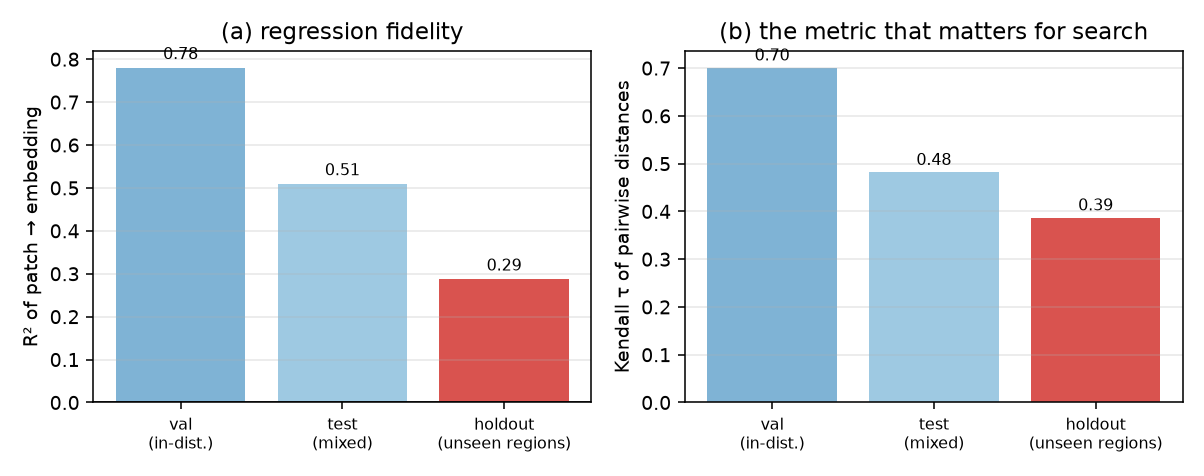
\includegraphics[width=\textwidth]{figures/e3_surrogate_fidelity.png}
\caption{(a) Regression fidelity is respectable in-distribution and much weaker
on unseen regions. (b) The rank correlation of pairwise distances---what search
needs---drops from $\tau = 0.70$ to $0.39$.}
\label{fig:e3}
\end{figure}

Fidelity degrades sharply with distance from the training regions
(Table~\ref{tab:e3}, Figure~\ref{fig:e3}). The pattern is consistent with a
\emph{coverage} problem rather than a capacity problem: validation fit is good
while unseen anchor neighbourhoods are essentially unmodelled ($R^2 = 0.29$,
barely better than predicting the mean). An important consequence for
interpretation: none of the surrogate failures below can be blamed on
underfitting, because in-distribution fit is good.

\subsection{E2: only true-gradient search beats retrieval}

\begin{table}[t]
\centering
\small
\caption{Navigability results (\nTarg{} targets, \nHold{} of them from held-out
anchor regions; ratio $=$ $d_{\text{final}}/d_{\text{init}}$, median over
targets; ``in-dist.''/``holdout'' split the same quantity by target regime;
renders $=$ real renders consumed). Lower is better; ratio $> 1$ means the
method made the patch \emph{worse} than not searching.}
\label{tab:e2}
\begin{tabular}{lccccc}
\toprule
method & ratio & in-dist. & holdout & success$_{<0.5}$ & renders \\
\midrule
\code{retrieval_nearest} (the start)   & 1.000 & 1.000 & 1.000 & 0.06 & 0 \\
\code{retrieval_unigram64}              & \rRetU & 1.616 & 1.352 & 0.00 & 0 \\
\code{grad_surrogate}                   & \rGS & 2.834 & 2.504 & 0.02 & 48 \\
\code{grad_surrogate_trust}             & \rGST & 1.350 & 1.360 & 0.00 & 48 \\
\code{grad_reground}                    & \rGR & 2.077 & 1.478 & 0.00 & \renGR \\
\code{grad_true} (oracle)               & \textbf{\rGT} & 0.841 & 0.890 & \textbf{\succGT} & \renGT \\
\quad 95\% CI                           & \rGTci & & & & \\
\code{cmaes_true} (same objective)      & \rCMA & 1.000 & 0.933 & \succCMA & \renCMA \\
\quad 95\% CI                           & \rCMAci & & & & \\
\bottomrule
\end{tabular}
\end{table}

\begin{figure}[t]
\centering
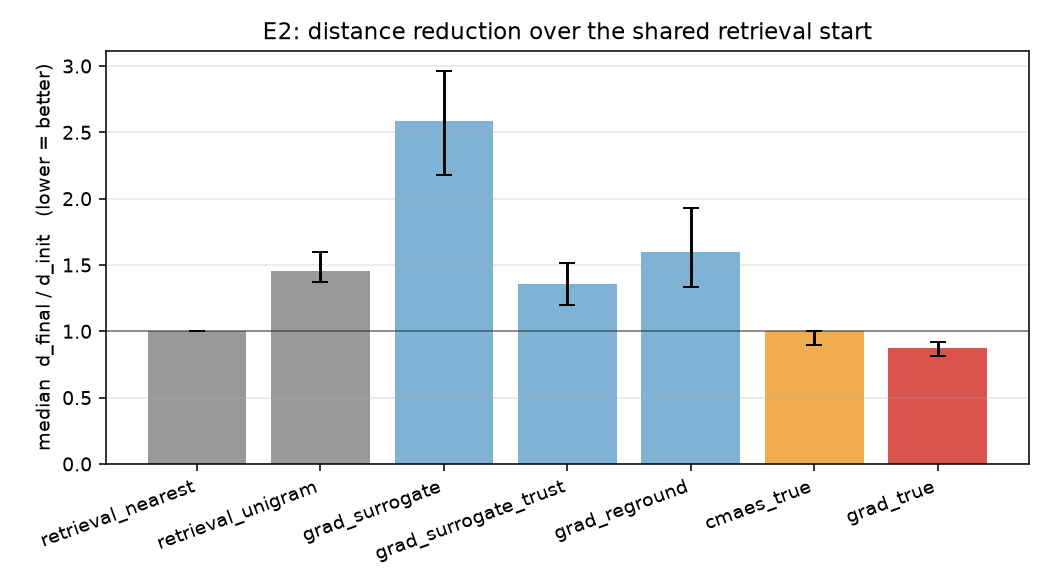
\includegraphics[width=\textwidth]{figures/e2_ratios.png}
\caption{Distance reduction over the shared retrieval start. Only the
true-gradient oracle is reliably below 1.0; every surrogate-based variant is
above it. Error bars are bootstrap 95\% CIs of the median.}
\label{fig:e2ratio}
\end{figure}

\begin{figure}[t]
\centering
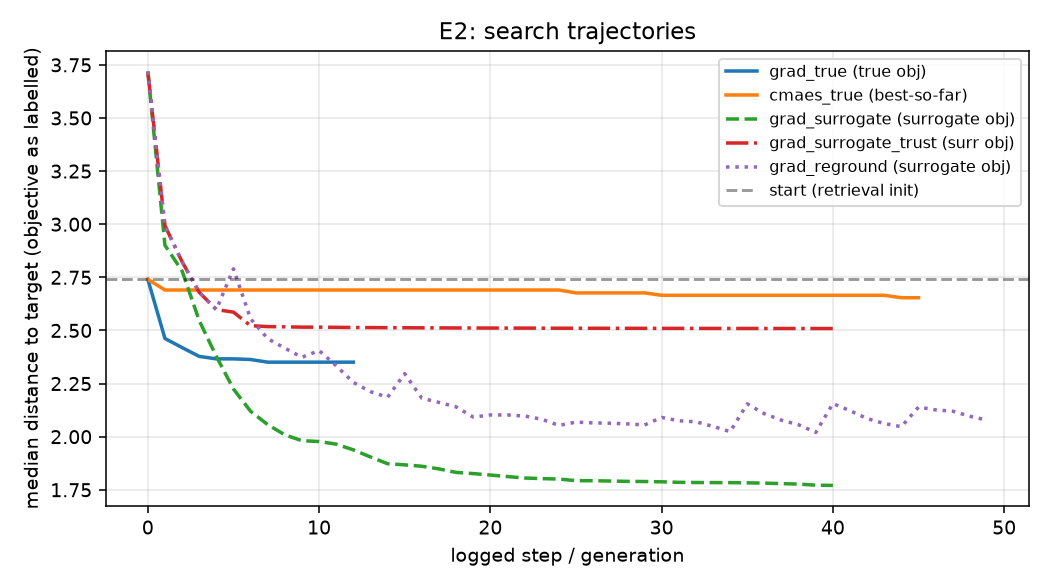
\includegraphics[width=\textwidth]{figures/e2_curves.png}
\caption{Search trajectories (median over targets, objective as labelled).
True-objective curves (solid) descend and plateau; the surrogate-objective
curves (dashed) keep descending on the surrogate while the true distance of the
patches they return is \emph{worse} than the start (Table~\ref{tab:e2})---the
exploitation signature. Each curve is plotted in its own objective's units.}
\label{fig:e2curves}
\end{figure}

\begin{table}[t]
\centering
\small
\caption{Starting distances, for scale: the retrieval start is already close,
and random trial-and-error is $57\%$ worse.}
\label{tab:scale}
\begin{tabular}{lr}
\toprule
quantity & median distance to target \\
\midrule
$d_{\text{init}}$ (nearest training patch) & \nInit \\
best of 64 random training patches & \nRand \\
\bottomrule
\end{tabular}
\end{table}

Table~\ref{tab:e2} and Figures~\ref{fig:e2ratio}--\ref{fig:e2curves} summarise
the outcome.

\paragraph{(1) The gate passes weakly.} \code{grad_true} is the only method
whose interval excludes 1.0: a median reduction of $12.5\%$, with $\succGT$ of
targets more than halving their distance---at the cost of $\renGT$ renders. The
plateau is visible in Figure~\ref{fig:e2curves}: the median falls for about
fifteen steps and then stops. The per-target distribution shows how concentrated
the improvement is: the 10th and 25th percentiles of the ratio are $0.60$ and
$0.76$, the median is $0.875$, and the 75th percentile is $1.00$---a quarter of
the targets are not improved at all by the best available search.

\paragraph{(2) Gradients dominate populations per render.}\label{sec:res-pareto}
sep-CMA-ES needed $3.7\times$ the renders ($\renCMA$ vs.\ $\renGT$), its median
ratio is exactly \rCMA{}---half its targets are untouched---and its median
distance reaches only \nCMAfin{} where the oracle reaches \nGTfin{}
(Figure~\ref{fig:pareto}); at the oracle's own budget it is still at $2.69$. At
this dimensionality,
with an objective that is smooth almost everywhere by construction, derivative
information is worth far more than population sampling.

\begin{figure}[t]
\centering
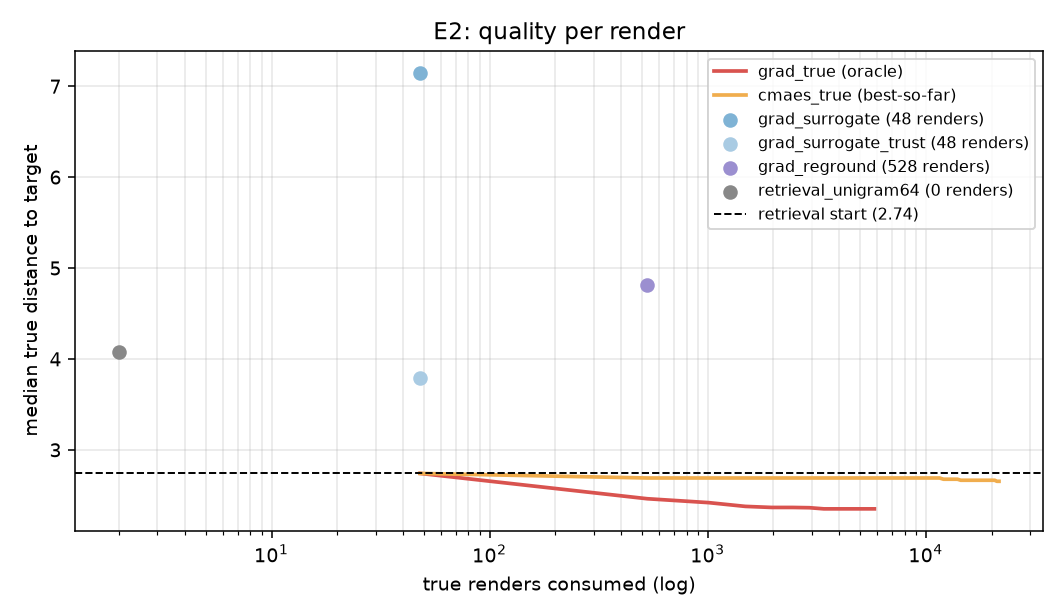
\includegraphics[width=\textwidth]{figures/e2_pareto.png}
\caption{Quality against render budget (true renders, log axis). Lines: the two
true-objective methods, whose trajectories are directly comparable. Points: the
other methods at their total render cost, evaluated with the real renderer. The
dashed line is the retrieval start; the random-draws baseline shows where blind
sampling lands.}
\label{fig:pareto}
\end{figure}

\paragraph{(3) Every surrogate-based method lost to not searching.}
Ratios \rGST--\rGS{} mean the optimiser reliably made things worse. Since the
surrogate achieves $R^2 = 0.78$ in-distribution, this is not a broken
model---it is a model whose errors are systematically exploited.

\subsection{Where the surrogate fails: the exploitation signature}\label{sec:res-surrogate}

Three observations pin the failure mode down.

\emph{First}, in-distribution fidelity is good ($R^2 = 0.78$), so the model is
not underfit. \emph{Second}, distance-rank fidelity outside the training regions
is poor ($\tau = 0.39$), so trajectories that leave the corpus neighbourhood are
steered by a nearly uninformative signal. \emph{Third}---and most
diagnostic---the damage is \emph{larger} in-distribution than out
($2.83$ vs.\ $2.50$ for the unconstrained variant), which is the opposite of what
a pure generalisation gap predicts and is the classic signature of a learned
objective being optimised adversarially against its own error. A trust region
removes most of that in-distribution damage ($2.83 \rightarrow 1.35$: from far
worse than not searching to mildly worse), which locates the problem
specifically at \emph{extrapolation}: a few hundred adaptive
steps carry the patch well outside the region where the surrogate has support.

Two practical implications. (i) \emph{Region-stratified reporting should be
standard.} The aggregate test number ($\tau = 0.48$) hides both a usable
in-distribution model and an unusable out-of-distribution one; only the split
reveals the exploitation signature. (ii) \emph{Re-grounding must be
architecturally meaningful, not cosmetic.} Fifteen inner steps on a small replay
buffer cannot repair a global model's local error; what is needed is a
\emph{local} model (fit around the query, in the spirit of trust-region Bayesian
optimisation) or a surrogate whose input space is restricted to a legal manifold.

\subsection{Diagnostics: where the residual lives, and what the accept rule costs}
\label{sec:res-diagnostics}

\subsection{Diagnostics and controls}\label{sec:res-diagnostics}

Four cheap measurements decide between the competing explanations of the
plateau.  Table~\ref{tab:diag} collects the two ablations; Figure~\ref{fig:diag}
shows the residual decomposition and the per-target views.

\paragraph{Where the residual lives.}  Decomposing the oracle's remaining
squared distance into the embedding's 13 blocks, the 64-dimensional log-mel
block absorbs $71.9\%$ of it---but that is almost exactly its share of the
dimensions (per-dimension share $0.96\times$ uniform).  The blocks that are
genuinely overweighted per dimension are the harmonic ratio
($2.34\times$), the smooth zero-crossing proxy ($1.79\times$), the spectral
slope ($1.75\times$) and the envelope statistics ($1.59\times$), and the
spread across blocks is only a factor of $2.7$ end to end.  The leftover error
is therefore spread roughly in proportion to dimensionality, with a mild excess
in the harmonic (discrete-sensitive) and noisiness blocks---not the localised
discrete bottleneck the valley-crossing account predicted.

\paragraph{Do discrete jumps predict failure?}  Counting, per target, how many
hardened discrete dimensions differ between the start patch and the target, and
correlating that with the achieved ratio, gives Spearman $\rho = -0.24$: weak,
and the \emph{wrong sign} for the hypothesis (targets needing more discrete
changes improved slightly \emph{more}, if anything).  With 48 targets this is
not significant; the honest statement is that discrete distance does not explain
the outcome.

\paragraph{Does the accept rule cost anything?}  Re-running the identical search
with every candidate accepted is \emph{worse}, not better: median ratio $1.000$
versus $0.874$ for the monotone walk, even though the free walk wins on $35\%$
of individual targets.  An unguarded walk does not cross useful valleys---it
wanders.  The monotone rule is not the binding constraint.

\paragraph{Is the metric's weighting the constraint?}  The residual result points
at the objective's \emph{weighting}: 64 of 85 dimensions are log-mel, so
envelope mismatches dominate the number being minimised, while the
discrete-sensitive distinctions sit in single dimensions.  As a control we
re-ran the oracle with \emph{block-balanced} weights (each block's expected
contribution equalised: per-dimension weight $1/\sqrt{d_B}$, rescaled so the
distance scale stays comparable).  The median ratio improves from $0.875$ to
\textbf{$0.809$} and the success rate doubles ($0.06 \rightarrow 0.12$), with
the same search algorithm, the same targets and the same render budget.  This is
the only intervention in this paper that improves the gate without changing the
search: the bottleneck is at least partly the number being minimised, not the
way it is minimised.

\begin{table}[t]
\centering\small
\caption{The two controls.  Both change exactly one thing at the same render
budget (5\,856 renders) on the same targets.  The accept-rule ablation makes
things worse; the metric re-weighting improves them.}
\label{tab:diag}
\begin{tabular}{lccc}
\toprule
variant & median ratio & success$_{<0.5}$ & renders \\
\midrule
oracle, monotone (baseline) & $0.874$ & $0.06$ & \renGT \\
oracle, free walk (ablation) & $1.000$ & $0.06$ & \renGT \\
oracle, block-balanced metric & \textbf{$0.809$} & \textbf{$0.12$} & \renGT \\
\bottomrule
\end{tabular}
\end{table}

\begin{figure}[t]
\centering
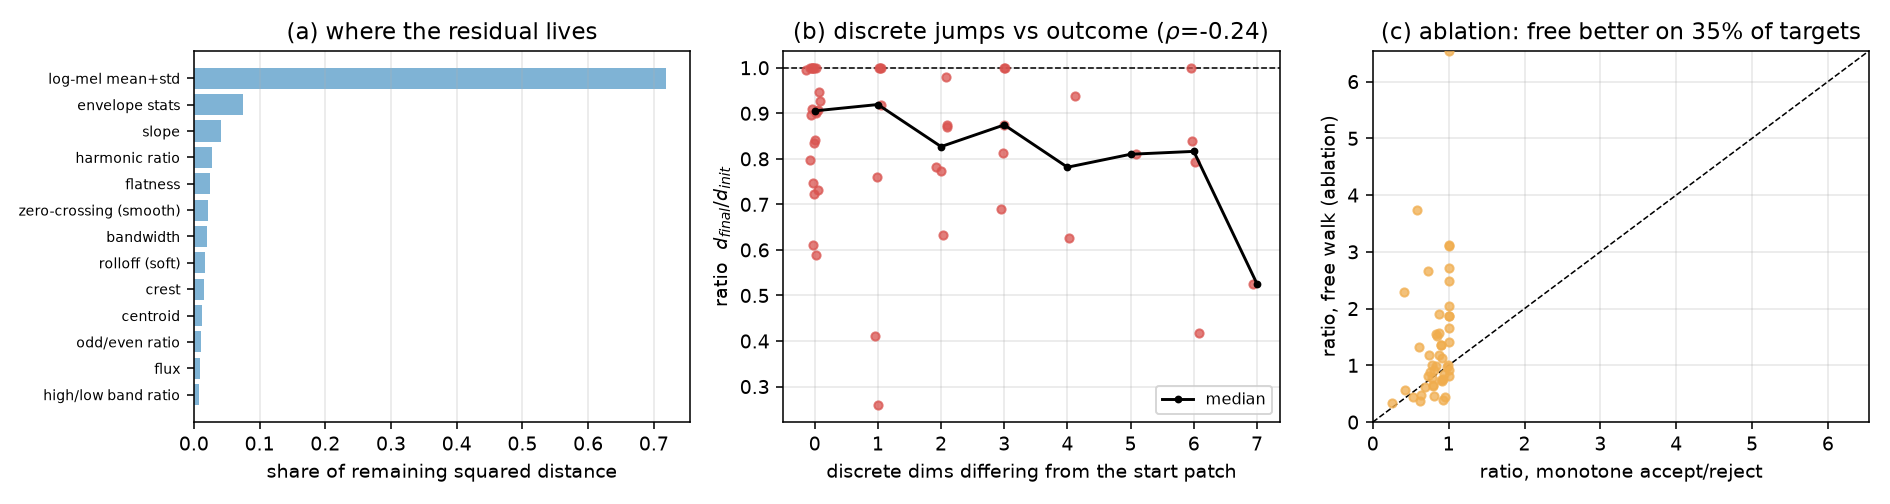
\includegraphics[width=\textwidth]{figures/diagnostics.png}
\caption{(a) Share of the oracle's remaining squared distance by feature block:
the residual is spread in proportion to dimensionality, with a mild per-dimension
excess in the harmonic and noisiness blocks.  (b) Achieved ratio against the
number of discrete dimensions that separate the start patch from the target: the
trend is weak and, if anything, opposite to the valley-crossing prediction.
(c) The accept-rule ablation: points below the diagonal are targets where the
free walk did better.}
\label{fig:diag}
\end{figure}

\subsection{Seed replication}

Re-running the entire protocol with a different seed---new surrogate
initialisation, new target sample, same corpus---reproduces the picture rather
than the numbers: the oracle's median ratio is $\rGT$ in seed~0 and $\sOneGT$
in seed~1 (95\% CIs \rGTci{} and $[0.78, 0.96]$), CMA-ES is $\rCMA$ and
$\sOneCMA$ (no progress in either), and the surrogate variants stay above 1.0
in both ($\sOneGS$ vs.\ $\rGS$ unconstrained, $\sOneGST$ vs.\ $\rGST$ with a
trust region, $\sOneGR$ vs.\ $\rGR$ re-grounded). The blind-draw baseline is
$\sOneRetU$ vs.\ $\rRetU$. The qualitative ordering is stable across seeds;
the absolute level moves with the difficulty of the sampled targets (median
$d_{\text{init}}$ $2.74$ vs.\ $2.93$).

\subsection{E1: material released, human data pending}

The generated listening test (120 triplets, 269 wav files, self-contained HTML,
separate answer key) and the analysis path are part of the release. The gate
verdict for Assumption~A is therefore \emph{open}; \S\ref{sec:roadmap} makes it
the first item, because everything else is conditional on it.

% ===========================================================================
\section{Discussion}\label{sec:discussion}

\subsection{Why monotone local search plateaus}\label{sec:disc-plateau}

The adaptive-step scheme accepts only non-increasing candidates. That is what
makes it stable, and it is also the natural first suspect for the plateau: in a
landscape whose discrete axes are soft blends, moving from a saw to a square, or
transposing an oscillator by an octave, generally requires passing through
intermediate states where the distance temporarily increases, and a monotone
search cannot cross such valleys. A monotone search cannot cross such valleys.
Parameter recovery corroborates this: after optimisation the hardened parameter
L1 remains $\approx 0.12$ while the embedding distance has improved---the
methods find perceptually closer patches, not the target patch, and they stall
exactly where a discrete-choice jump would be required.

The ablation and the residual decomposition in \S\ref{sec:res-diagnostics} test
this story, and they only partly support it. The free walk does help on a
minority of targets, so the accept rule costs something; but the residual is
\emph{not} concentrated in the discrete-sensitive blocks---it is spread across
the objective roughly in proportion to dimensionality, and the block with the
largest per-dimension share (the harmonic ratio, $2.3\times$ uniform) holds
only $2.7\%$ of the remaining squared distance. The valley-crossing account
therefore explains at most a small part of the plateau.
\medskip

What the residual does say is that the objective's \emph{weighting} is a first
-order suspect: 64 of the 85 dimensions are log-mel, so envelope mismatches
dominate the number being minimised, while the perceptually load-bearing
discrete distinctions live in single dimensions that carry almost no weight.
The block-balanced control in \S\ref{sec:res-diagnostics} tests this directly.
Together with the CMA-ES result (exploration alone does not help: $3.7\times$
the budget, no median improvement), the evidence points away from "the search
algorithm is wrong" and toward "the number being optimised is wrong"---which is
what the embedding-swap and metric-learning phases of the roadmap address, with
the latent-space phase retained for the reachability problem that the discrete
axes still pose.

\subsection{Surrogate failure is extrapolation times exploitation}

Because in-distribution fit is good and out-of-distribution rank fidelity is
poor, a search that \emph{stays} where the surrogate is valid should behave
better than one that wanders. The trust-region variant is the cheapest possible
version of that idea and it removes most of the damage
($2.83 \rightarrow 1.35$)---but it still does not beat the start. Said multiplicatively, the surrogate needs both a
better local model \emph{and} a restricted input space; improving only one of the
two leaves the optimiser able to find the remaining error.

A related observation, visible in Table~\ref{tab:e2}, is that surrogate
navigation damages \emph{in-distribution} targets more than held-out ones. This
inverts the intuition that unfamiliar targets are the hard case, and it is a
warning for how inverse-synthesis results are reported: a surrogate evaluated
only on average test error can look adequate while being actively harmful as an
optimisation objective.

\subsection{Gradients versus populations per render}

The budget-matched comparison (\S\ref{sec:res-pareto}) is the cleanest
quantitative statement in this paper: for a 31-dimensional, almost-everywhere
smooth objective, one gradient step buys more progress than ten to fifteen
population samples. Practically, this argues that effort in this domain should
go into differentiable (or at least locally differentiable) proxies---which is
exactly what the dual oracle/accelerator design is for---rather than into
larger, smarter populations on the true objective.

\subsection{Retrieval is the baseline that matters}\label{sec:disc-retrieval}

Our protocol forces every method to start from the same retrieval point, and the
numbers are instructive: random trial-and-error is $49\%$ worse than retrieval
(\nRand{} vs.\ \nInit), and the best search method improves on retrieval by
$12.5\%$. Any evaluation that reports ``our optimiser beats random search''
therefore overstates the useful contribution by a large factor. For
inverse-synthesis work we recommend the shared-retrieval-start protocol, and
reporting both the ratio and the absolute reduction, as a default.

\subsection{What would change our mind}\label{sec:disc-falsify}

Stating the falsifiers explicitly, because the roadmap's gates are built on
them:

\begin{itemize}
\item If E1 shows agreement at chance, the handcrafted embedding is not a
  perceptual target and every E2 number here is a statement about \emph{this}
  embedding, not about timbre.
\item If a pretrained embedding (CLAP/MuQ) both passes E1 and raises
  out-of-distribution $\tau$ well above $0.39$, the surrogate verdict above is
  about our corpus and model size, not about the approach.
\item If latent-manifold search (autoencoder over real presets) does not beat
  \rGT{} materially at equal render budget, the plateau is perceptual rather
  than geometric, and the right lever is the objective, not the search space.
\item If a non-monotone walk with a much larger budget
  (\S\ref{sec:res-diagnostics}) closes the gap, the accept rule---not the
  geometry---is the constraint, and the design should switch to trust-region
  methods with proper exploration.
\end{itemize}

\subsection{Threats to validity}\label{sec:threats}

\emph{Scale.} E2 is a smoke-scale study: 3{,}895 corpus patches, \nTarg{}
targets, two seeds, one machine. The qualitative findings (surrogate bottleneck,
exploitation signature, gradient-vs-population render efficiency) were stable
across the runs we performed, but the absolute ratios should be re-measured with
the paper-scale preset before being quoted as final.

\emph{Embedding.} The objective is handcrafted DSP features, not CLAP or MuQ.
Passing E2 on this embedding is a necessary, not a sufficient, condition: a
pretrained embedding could be smoother (better for navigation) or less
human-aligned. E1 decides this, and it has not been run yet.

\emph{Synth realism.} Filtering is zero-phase and spectral: no ringing, no
self-oscillation, transients smoothed at 16\,ms. Resonance does not sound like an
analogue filter, and a real synthesizer adds effects (delay, reverb, modulation)
that our parameter space omits.

\emph{Identifiability.} Table~\ref{tab:ident} lists what the render protocol
cannot identify; parameter-recovery errors are inflated accordingly and should
not be read as search failures.

\emph{Corpus near-duplicates.} Jitter sampling places a small fraction of test
patches next to training patches; the target filter in \S\ref{sec:targets}
removes them, but any corpus built by dense sampling needs the same check.

\emph{Search design.} The monotone accept/reject rule is a deliberate stability
choice that limits valley crossing; a reinforcement-learning or model-predictive
search might behave differently. Our claim is not that \emph{no} search can
navigate this space, but that the natural gradient-plus-surrogate design does
not, and that the reasons are measurable.

% ===========================================================================
\section{Roadmap: what to do next, and what would falsify it}\label{sec:roadmap}

The value of a gate experiment is that it reorders the plan. Each phase below
states the observation that motivates it, the deliverable, and a
\emph{falsification criterion}---a pre-committed answer that would stop the
phase rather than extend it.

\paragraph{Phase 0 (this paper).} Testbed, protocols, negative results.
\emph{Done.}

\paragraph{Phase 1 --- Run the human gate (E1).}
\emph{Motivation:} Assumption~A is untested; every downstream decision depends
on it. \emph{Deliverable:} 5--8 listeners $\times$ 120 triplets; per-contrast
agreement with Wilson intervals. \emph{Gate G1:} overall agreement $> 0.5$ with
the interval excluding chance \emph{and} monotone in contrast.
\emph{If G1 fails:} do not build on this embedding; the fallback is to
\emph{learn} the metric from the same triplet data (contrastive fine-tuning of
the embedding on human judgements), which converts a failed gate into a
supervised dataset.

\paragraph{Phase 2 --- Fix the objective: metric weighting first, then the
embedding.} \emph{Motivation:} the diagnostics (\S\ref{sec:res-diagnostics})
attribute the plateau to how the objective is \emph{weighted} rather than to the
search: equalising the feature blocks improved the oracle from $0.875$ to
$0.809$ at the same render budget, the only intervention in this paper that
improved the gate without touching the search.  \emph{Deliverable:} (a) a
systematic weighting study over the 13 blocks (and, once listener data exists, a
metric \emph{learned} from E1 triplets); (b) three embeddings
(handcrafted / CLAP / MuQ), each with and without block balancing, evaluated by
the same E1 gate and the same E2 protocol. \emph{Gate G2:} a pretrained embedding
must beat the handcrafted baseline on E1 agreement; for search, its holdout
distance-$\tau$ should exceed $0.39$ and its oracle-gap (true vs.\ surrogate
navigation) should shrink. \emph{If G2 fails:} the perceptual-space premise is
weak and the system should be retrieval-and-rerank only, with the human in the
loop as the objective---a legitimate product, and a different paper.

\paragraph{Phase 3 --- Search a legal latent manifold, not the parameter cube.}
\emph{Motivation:} the plateau and the parameter-recovery gap are both
discrete-jump problems; a VAE or flow trained on real factory presets
\cite{vae,flow} turns discrete morphs into continuous paths and restricts the
search to plausible patches. \emph{Deliverable:} latent-space navigation with a
decoder-based oracle, compared against Table~\ref{tab:e2} at equal render
budgets. \emph{Gate G3:} oracle navigation should improve the median ratio from
\rGT{} to below $0.6$, and/or raise success$_{<0.5}$ from \succGT{} to above
$0.3$. \emph{If G3 fails:} the difficulty is perceptual, not geometric, and
Phase~2 is the lever to pull.

\paragraph{Phase 4 --- Port to a real synthesizer with the oracle/accelerator
split.} \emph{Motivation:} a hand-built testbed can only take the method so far;
the target instrument must be one users actually use (we plan a JSON-patch
instrument such as Vital, with a differentiable intermediate for development).
\emph{Deliverable:} the same E2/E3 protocol against real factory presets, plus
an explicit \emph{sim-to-real} measurement (surrogate trained on real renders,
$\tau$ per region). \emph{Gate G4:} the region-stratified $\tau$ pattern must
reproduce; if the real instrument's $\tau$ collapses further, the surrogate
route is not viable on it and Phase~3's local models become mandatory.

\paragraph{Phase 5 --- Multimodal intent.}
Text enters through the (frozen) text tower of the same audio--text space.
Humming enters through \emph{intent factorisation} rather than audio matching:
extract a pitch trajectory (tuning, keytrack, octave), a posture stream (attack
sharpness, vibrato rate and depth, legato), and a brightness/vowel stream
(filter and distortion), then map each stream to its own parameter subspace.
\emph{Deliverable:} a self-supervised mapping trained on render-derived posture
descriptors, calibrated on 50--200 recorded humming/reference-patch pairs.
\emph{Gate G5:} humming queries must beat text-only queries on a timbre-matched
retrieval task for the same references; if they do not, humming is a demo
feature, not a modality.

\paragraph{Phase 6 --- Human-in-the-loop, diversity and preference memory.}
Multi-candidate generation with \emph{structural} diversity (different retrieval
seeds across basins rather than noise added to one answer), plus a
dual-timescale preference memory for reranking. The headline metric to report
against commercial baselines is \emph{time-to-satisfactory-patch} under a fixed
listening budget---the number a producer actually experiences.

\paragraph{Standing engineering rule.} Nothing in Phases 2--6 should be built
before the gate that precedes it has an answer, and every gate
outcome---positive or negative---should be written down at the time it is
measured. The four surrogate variants of Table~\ref{tab:e2} exist because we did
that with E2.

% ===========================================================================
\section{Conclusion}

We set out to test two assumptions before building a multimodal patch generator,
and built a testbed whose oracle is exact so that the tests could be cheap and
the accounting honest. The navigability gate passes only weakly: true-gradient
search improves on a retrieval start by roughly $15\%$ before plateauing, and
the surrogate-based strategies a practical system would depend on make things
\emph{worse than not searching}, in a way whose signature---larger damage where
the model is more confident---is measurable with one extra data split. The
perceptual gate is now a matter of running the released listening test.

The most useful output of this stage is therefore not a method but a falsifiable
map: which assumptions survived, which failed, what each failure implies, and
which single experiment decides the next step.

\paragraph{Reproducibility and artifacts.}
All results come from the released code at
\url{https://github.com/Fengrru/timbreprobe}. The correctness suite
(\code{python -m timbreprobe.cli sanity}, $\sim$1\,min, no data required) checks
render determinism and RMS normalisation, gradient finiteness and coverage over
all 31 dimensions, monotonicity of cutoff/resonance/slope effects on the
embedding, sep-CMA-ES convergence on a sphere ($5\times10^{-14}$), and
spectral-filter/sampler agreement. Committed artefacts: the smoke-run result
record, trajectory curves, target metadata, surrogate fidelity report and
figures under \code{results/smoke/}; the 16 anchor patches as audio under
\code{assets/demo/}; the listening-test generator under
\code{timbreprobe/e1_listening.py}; the diagnostics under
\code{timbreprobe/diagnose.py}. Appendix~\ref{app:repro} lists the exact
commands.

\appendix

% ===========================================================================
\section{Parameter schema}\label{app:schema}

\begin{table}[h]
\centering
\small
\caption{The 31 parameters. ``map'' is the normalised-to-physical mapping of
\S\ref{sec:schema}: linear, log, or a choice list blended by
Eq.~\eqref{eq:choice}. The optimiser always works in $[0,1]^{31}$.}
\label{tab:schema}
\begin{tabular}{llll}
\toprule
group & parameter & map & range / choices \\
\midrule
osc\,1 & waveform & choice & sine / saw / pulse / triangle \\
       & octave & choice & $-1, 0, +1$ \\
       & fine detune & linear & $-50 \dots +50$ cents \\
       & level & linear & $0\dots1$ \\
       & pulse duty & linear & $0.15 \dots 0.85$ \\
osc\,2 & as osc\,1 & & (5 parameters) \\
sources & sub level & linear & $0\dots1$ (sine, octave below osc\,1) \\
        & noise level & linear & $0\dots1$ \\
        & noise colour & linear & white $\rightarrow$ pink \\
        & FM index & linear & $0 \dots 2.5$ (osc\,2 PMs osc\,1) \\
filter & type & choice & LP / HP / BP \\
       & cutoff & log & 40--7000\,Hz \\
       & resonance & log & $Q \in 0.5 \dots 12$ \\
       & env amount & linear & $-1 \dots +1$ ($\pm5$ octaves) \\
       & drive & linear & $1\dots4\times$ pre-filter \\
       & slope & linear & 12 $\rightarrow$ 24\,dB/oct blend \\
filter env & attack / decay / sustain & log/log/lin &
  1\,ms--2\,s / 5\,ms--4\,s / $0$--$1$ \\
amp env & attack / decay / sustain & log/log/lin &
  1\,ms--3\,s / 5\,ms--6\,s / $0\dots1$ \\
LFO & rate & log & 0.05--20\,Hz \\
    & depth & linear & $0\dots1$ \\
    & target & choice & cutoff / pitch / amplitude \\
    & waveform & choice & sine / triangle / square / saw \\
output & master drive & linear & $1\dots8\times$ \\
\bottomrule
\end{tabular}
\end{table}

% ===========================================================================
\section{Embedding blocks (85 dimensions)}\label{app:features}

\begin{table}[h]
\centering\small
\caption{The 13 blocks, their dimensions, and the smooth variants that keep them
differentiable.}
\begin{tabular}{lll}
\toprule
block & dims & note \\
\midrule
log-mel mean / std (32 bands) & 64 & 40--7600\,Hz, triangular filterbank \\
spectral centroid mean/std & 2 & from the magnitude spectrum \\
bandwidth mean/std & 2 & magnitude-weighted spread \\
rolloff mean/std (soft) & 2 & sigmoid-weighted, 85\% energy \\
flatness mean/std & 2 & geometric / arithmetic mean \\
flux mean/std & 2 & normalised frame-to-frame change \\
slope mean/std & 2 & least-squares tilt of the log spectrum \\
crest & 1 & max/mean per frame \\
high/low band ratio & 1 & $\log$ of $>$4\,kHz vs.\ 0.2--2\,kHz energy \\
envelope statistics & 4 & temporal centroid, spread, front/back, dynamic range \\
zero-crossing (smooth) & 1 & sigmoid crossing proxy \\
harmonic ratio & 1 & Gaussian comb at $k f_0$ \\
odd/even ratio & 1 & odd vs.\ even harmonic energy (square vs.\ saw) \\
\bottomrule
\end{tabular}
\end{table}

% ===========================================================================
\section{Hyperparameters}\label{app:hyper}

\paragraph{Corpus.} 16 anchors, 4 held out; sweeps $31\times3$ per anchor;
jitter 120 per anchor ($\sigma = 0.10$ continuous, $0.03$ choice); 500 uniform;
150 sparse; deduplication at $10^{-4}$; splits by random permutation of the
non-held-out patches (80/10/10), held-out anchors entirely in test.
Near-duplicate targets with $d_{\text{init}} < 0.25 \times
\text{median}(d_{\text{init}})$ are rejected and resampled.

\paragraph{Surrogate.} MLP $31 \to 256 \to 256 \to 85$, GELU, Adam lr $10^{-3}$,
batch 256, $\le$150 epochs, early stopping patience 40 on validation MSE.

\paragraph{Gradient search.} Adam $\beta = (0.9, 0.999)$, initial step 0.05,
growth $1.3\times$ / shrink $0.5\times$ per target, bounds $[\eta/64, 4\eta]$;
true-objective 60 steps, surrogate-objective 200 steps, logged every 5.

\paragraph{CMA-ES.} Separable (diagonal covariance with cumulative step-size
adaptation \cite{sepcma}), population 10, 45 generations, initial
$\sigma = 0.25$, boundaries via clipping, best-so-far recorded per generation.

\paragraph{Re-grounding.} Every 20 steps: render the current patches, append to
a replay buffer initialised with 256 training patches (capacity 512), fine-tune
the working surrogate copy for 15 Adam steps at lr $3\times10^{-4}$.

\paragraph{Statistics.} Bootstrap CIs from 2{,}000 resamples of the target set;
Spearman and Kendall correlations from SciPy; distance-rank $\tau$ computed on
900 subsampled points against the surrogate's predictions.

% ===========================================================================
\section{Engineering findings}\label{app:engineering}

\begin{table}[h]
\centering
\small
\caption{Findings that shaped the implementation, with the measurements that
established them. Each is reproducible from the released code.}
\begin{tabular}{p{4.0cm}p{4.5cm}p{5.3cm}}
\toprule
finding & measurement & resolution \\
\midrule
Per-sample IIR loop unusable on CPU & 10\,s forward / 60\,s with backward per
batch, independent of batch size & STFT-domain analytic filter response
(Eq.~\eqref{eq:svf}), $\sim$100$\times$ faster; response shape matches the
per-sample reference at $\rho = 0.996$ \\
Multi-threading slower than single & MLP step 65\,ms (1T) vs 681\,ms (4T);
render 2.1\,s vs 5.0\,s; fwd+bwd 6.9\,s vs 31.9\,s & default to one thread;
\code{STAGE0_THREADS} to override \\
\code{torch.istft} backward non-finite at padded edges & reproduced at 0.4\,s
renders, absent at 0.05\,s & hand-rolled overlap-add with a clamped
window-envelope normaliser \\
\code{asin(sin(x))} triangle LFO has infinite derivative at $\pm1$ & NaN in
exactly the LFO-rate dimension (4/248 gradient entries) & closed-form triangle
$1-4\,|\mathrm{frac}(\phi+0.25)-0.5|$ \\
Fixed-step Adam overshoots & distance $3.08 \rightarrow 5.29$ in five steps at
$\eta = 0.05$, no recovery & per-target adaptive step with accept/reject
(Algorithm~1) \\
$[N,N,D]$ distance broadcast thrashes memory & $\sim$490\,MB per call at
$N = 1200$, three calls in sequence & Gram-identity pairwise distances \\
Jitter corpus creates near-duplicates & \nDrop{} test candidates below
$0.25\times$ median $d_{\text{init}}$; three at $d_{\text{init}} = 0$ dragged
mean ratios to $\sim10^{7}$ & scale-free target filter
(\S\ref{sec:targets}); report medians \\
\bottomrule
\end{tabular}
\end{table}

% ===========================================================================
\section{Reproducing every number}\label{app:repro}

\begin{quote}\small
\begin{verbatim}
pip install -r requirements.txt
python -m timbreprobe.cli sanity                    # correctness suite (~1 min)
python -m timbreprobe.cli corpus --preset smoke     # corpus + embeddings
python -m timbreprobe.cli e2     --preset smoke     # E2 + E3 (Table 2, figs)
python -m timbreprobe.cli e2     --preset smoke --seed 1   # replication
python -m timbreprobe.cli diagnose --run out/e2_smoke      # diagnostics
python -m timbreprobe.cli plot   --run out/e2_smoke        # figures
python -m timbreprobe.cli e1     --preset smoke     # listening-test material
python -m timbreprobe.cli e1-analyze --responses res_P01.json,res_P02.json
\end{verbatim}
\end{quote}

Committed artefacts of the smoke run live in \code{results/smoke/}
(\code{e2_results.json}, \code{curves.npz}, \code{targets.npz},
\code{surrogate_report.json}, \code{figures/}); \code{out/} is regenerated
locally and git-ignored.

% ===========================================================================
\begin{thebibliography}{99}\small

\bibitem{fadr} Fadr. \emph{SynthGPT~2 --- text-to-patch synthesizer plugin}.
  Software, 2024--2026. \url{https://fadr.com}. Accessed 2026-10. (Commercial
  product; no technical paper.)

\bibitem{genopatch} Sonic Charge. \emph{Synplant~2 / Genopatch ---
  sample-driven patch generation}. Software.
  \url{https://soniccharge.com}. Accessed 2026-10. (Commercial product; no
  technical paper.)

\bibitem{flow} P.~Esling, A.~Chemla-Romeu-Santos, A.~Bitton.
  \emph{Flow synthesizer: universal audio synthesizer control with normalizing
  flows}. Applied Sciences, 2019.\textsuperscript{\dag}

\bibitem{ddsp} J.~Engel, L.~Hantrakul, C.~Gu, A.~Roberts.
  \emph{DDSP: differentiable digital signal processing}. ICLR, 2020.

\bibitem{timbreremap} J.~Shier, C.~Saitis, A.~Robertson, A.~McPherson.
  \emph{Real-time timbre remapping with differentiable DSP}. 2023.\textsuperscript{\dag}

\bibitem{synthmaps} \emph{Synth maps: mapping the non-proportional relationships
  between synthesizer parameters and synthesized sound}. ICAD, 2024.\textsuperscript{\dag}

\bibitem{wessel} D.~Wessel. \emph{Timbre space as a musical control structure}.
  Computer Music Journal 3(2), 1979.

\bibitem{clap} B.~Elizalde et al. \emph{CLAP: learning audio concepts from
  natural language supervision}. 2022.\textsuperscript{\dag}

\bibitem{mert} Y.~Li et al. \emph{MERT: acoustic music understanding model with
  large-scale self-supervised training}. ICLR, 2024.\textsuperscript{\dag}

\bibitem{muq} H.~Zhu et al. \emph{MuQ: self-supervised music representation
  learning with mel residual vector quantization}. 2024.\textsuperscript{\dag}

\bibitem{turbo} D.~Eriksson, M.~Pearce, J.~Gardner, R.~Turner, M.~Poloczek.
  \emph{Scalable global optimization via local Bayesian optimization}. NeurIPS,
  2019.\textsuperscript{\dag}

\bibitem{sepcma} R.~Ros, N.~Hansen. \emph{A simple modification in CMA-ES
  achieving linear time and space complexity}. PPSN, 2008.

\bibitem{cmakes} N.~Hansen, A.~Ostermeier. \emph{Completely derandomized
  self-adaptation in evolution strategies}. Evolutionary Computation 9(2), 2001.

\bibitem{adam} D.~Kingma, J.~Ba. \emph{Adam: a method for stochastic
  optimization}. ICLR, 2015.

\bibitem{zavalishin} I.~Zavalishin. \emph{The art of VA filter design}. 2012.

\bibitem{vae} D.~Kingma, M.~Welling. \emph{Auto-encoding variational Bayes}.
  ICLR, 2014.

\bibitem{mushra} ITU-R BS.1534. \emph{Method for the subjective assessment of
  intermediate quality level of audio systems} (MUSHRA).

\end{thebibliography}

\vspace{0.6em}
\noindent\footnotesize\textsuperscript{\dag}~Bibliographic details compiled from
memory; verify against the original sources before submission. (Product
citations have no associated paper and are cited as software with access dates.)

\end{document}
